\section{Introduction}\label{sec:introduction}
\IEEEPARstart{W}{e} are in an era of data explosion --- 2.5 quintillion bytes of data are created every day according to IBM's report\footnote{http://www-01.ibm.com/software/data/bigdata/}.
{\color{black}
In \textit{industry 4.0}, an increasing number of IoT sensors are embedded in the industrial production line \cite{lade2017manufacturing}.
During the manufacturing process, the information about the assembly lines, stations, and machines is continuously generated and collected.
Using distributed computing frameworks to analyze industrial big-data is an inevitable trend \cite{lee2014service}.
% \cite{ibmreport}.
% These data come from a variety of industry, e.g., records in industrial production, digital pictures and videos in social networks, and sensors used for Internet of Things (IoT).
% These data come from a variety of industries, e.g., e-commerce, telecommunications, media, retail customers and social networks.
% \cite{chen2012interactive}.
% Whether the data is generated from industrial production or social networks, the analysis methods are almost MapReduce-related\cite{lv2017next}.
% Nowadays, the real challenge of big data is not how to collect it, but how to manage it logically and efficiently\cite{lv2017next}.
Several sophisticated frameworks are used in industrial big-data analysis such as Hadoop MapReduce\footnote{http://hadoop.apache.com/}, Spark\footnote{https://spark.apache.org/}, and Storm\footnote{http://storm.apache.com/}.
% The analysis method for these industrial big data mainly relies on MapReduce-liked frameworks, such as Hadoop MapReduce\footnote{http://hadoop.apache.com/}, Spark\cite{spark}, and Storm\footnote{http://storm.apache.com/}.
% Recent years have witnessed the widespread use of sophisticated frameworks, such as Hadoop MapReduce\footnote{http://hadoop.apache.com/}, Dryad \cite{dryad}, Spark \cite{spark}, and Apache Tez \cite{tez}.
Industrial big-data is more structured, correlated, and ready for analytics than traditional big-data, because industrial big-data is generated by automated equipment \cite{basanta2018efficient, lv2017next}.
}

{\color{black}
According to a cross-industry study \cite{chen2012interactive}, both industrial and traditional big-data share a characteristic during analytical processing --- a small fraction of the daily workload uses well over 90\% of the cluster’s resources, and these workloads often contain a huge shuffle size. 
According to another MapReduce trace analysis from Facebook, the shuffle phase accounts for $33\%$ of the job completion time on average, and up to $70\%$ in shuffle-heavy jobs \cite{managing}.
The shuffle phase is crucial and heavily affecting the end-to-end application performance.
Most of the popular frameworks define jobs as directed acyclic graphs (DAGs), such as map-reduce pipeline in Hadoop MapReduce, lineage of resilient distributed datasets (RDDs) in Spark, vertices and edges in Dryad \cite{dryad}, and Tez\footnote{https://tez.apache.org/}, etc.
Despite the differences among data-intensive frameworks, the shuffle phase is always essential as communication between successive computation stages.
}

\begin{figure}
	\centering
	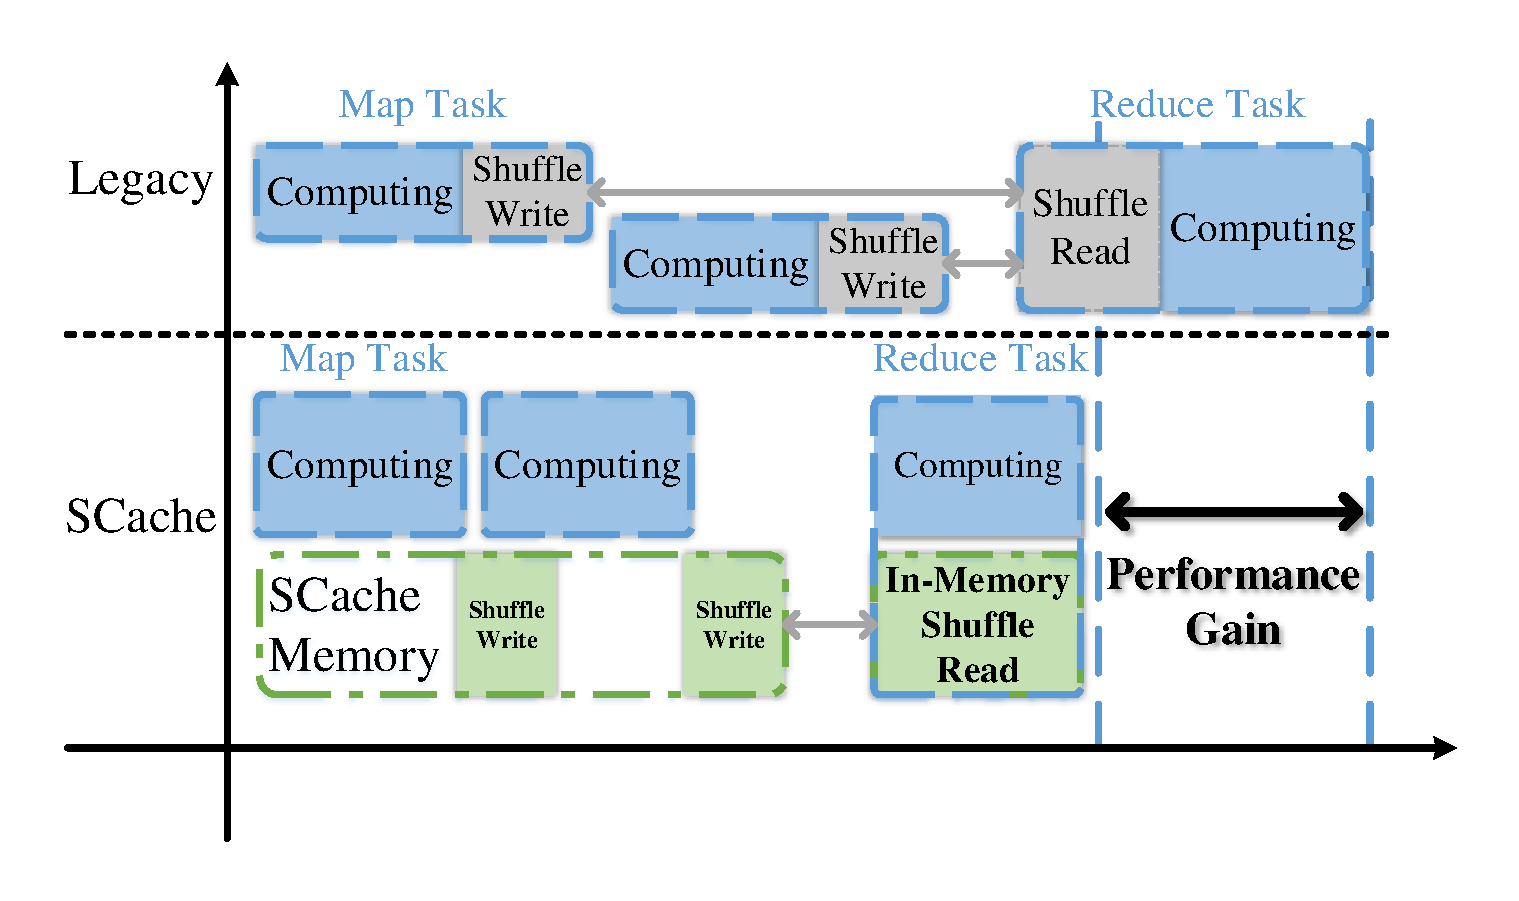
\includegraphics
		[width=1\linewidth]
		{fig/workflow}
	\caption{Workflow Comparison between Legacy DAG Computing Frameworks and Frameworks with SCache}
	\label{fig:workflow}
\end{figure}
{\color{black}
Although continuous efforts of performance optimization have been made among a variety of computing frameworks\cite{chen2017parallel, sync, tachyon, heintz2016end, cheng2017improving, wasi2017comprehensive}, the shuffle phase is often poorly optimized in practice.
In particular, we observe that one major deficiency lies in the coupled scheduling among different system resources.
}
As Figure \ref{fig:workflow} shows, the \textit{shuffle write} is responsible for writing intermediate results to disk, which is attached to the tasks in ancestor stages (i.e., map task).  
And the \textit{shuffle read} fetches intermediate results from remote disks through network, which is commonly integrated as part of the tasks in descendant stages (i.e., reduce task). 
Once scheduled, a fixed bundle of resources (i.e., CPU, memory, disk, and network) named \textit{slot} is assigned to a task, and the resources are released only after the task finishes.
Such task aggregation together with the coupled scheduling effectively simplifies task management.
However, since a cluster has a limited number of slots, attaching the I/O intensive shuffle phase to the CPU/memory intensive computation phase results in a poor multiplexing between computational and I/O resources.

Moreover, the shuffle read phase introduces all-to-all communication pattern across the network, and such network I/O procedure is also poorly coordinated.
Note that the shuffle read phase starts fetching data only after the corresponding reduce task starts.
Meanwhile, the reduce tasks belonging to the same execution phase are scheduled at the same time by default. 
As a result, all the corresponding reduce tasks start fetching shuffle data almost simultaneously.
Such synchronized network communication causes a burst demand for network I/O, which in turn greatly enlarges the shuffle read completion time. 
To desynchronize the network communication, an intuitive way is to launch some tasks in the descendent stage earlier, such as "slow-start" from Hadoop MapReduce.
{\color{black}
However, such early-start is by no means a panacea.
This is mainly because the early-start always introduces an extra early allocation of the slot leading to a slow execution of the current stage.
% However, such early-start has several deficiencies.
% First, the early-start always introduces an extra early allocation of the slot leading to a slow execution of the current stage.
% Second, the early-start can not fully overlap the shuffle phases and the descendent stage. Due to the shuffle phases are coupled with the reduce phases and the size of slots is limited, only parts of reduce tasks can be early-start. 
% Last but not least, it is hard to find the optimal time to begin the early-start. If too early, the descendent stages are not ready to output enough intermediate data for the shuffle. If too late, the idle network resource is wasted.
}

% We note that the above deficiencies generally exist in most of the DAG computing frameworks. 
% As a result, even though we can effectively resolve the above deficiencies by modifying one framework, updating one application at a time is impractical given the sheer number of computing frameworks available today.

Can we efficiently optimize the data shuffling without significantly changing DAG frameworks?
In this paper, we answer this question in the affirmative with S(huffle)Cache, an open source\footnote{https://github.com/frankfzw/SCache} plug-in system which provides a shuffle-specific optimization for different DAG computing frameworks.
Specifically, SCache takes over the whole shuffle phase from the underlying framework by providing a cross-framework API for both shuffle write and read.
SCache's effectiveness lies in the following two key ideas.
First, SCache decouples the shuffle write and read from both map and reduce tasks.
Such decoupling effectively enables more flexible resource management and better multiplexing between the computational and I/O resources.
In addition, SCache pre-schedules the reduce tasks without launching them and pre-fetches the shuffle data. 
% for the reduce tasks.
Such pre-scheduling and pre-fetching effectively overlap the network transfer time, desynchronize the network communication, 
and avoid the extra early allocation of slots.

The workflow of a DAG framework with SCache is presented in Figure \ref{fig:workflow}. 
SCache replaces the disk operations of shuffle write by the memory copy in map tasks. 
The slot is released after the memory copy. 
The shuffle data is stored in the reserved memory of SCache until all reduce tasks are pre-scheduled. 
Then the shuffle data is pre-fetched according to the pre-scheduling results.  
The application-context-aware memory management caches the shuffle data in memory before launching the reduce task.
By applying these optimizations, SCache can help the DAG framework achieve a significant performance gain.  

The main challenge to achieve this optimization is \textit{pre-scheduling reduce tasks without launching}. 
First, the complexity of DAG can amplify the defects of na\"{i}ve scheduling schemes. 
In particular, randomly assigning reduce tasks might result in a collision of two heavy tasks on one node. 
This collision can aggravate data skew, thus hurting the performance. 
Second, pre-scheduling without launching violates the design of most frameworks that launch a task after scheduling.
To address the challenges, we propose a heuristic task pre-scheduling scheme with shuffle data prediction and a task co-scheduler (Section \ref{opt}).

Another challenge is the \textit{in-memory data management}. 
To prevent shuffle data touching the disk, SCache leverages extra memory to store the shuffle data. 
To minimize the reserved memory while maximizing the performance gain, we propose two constraints: all-or-nothing and context-aware (Section \ref{impl}).

{\color{black}
We also propose a new performance model called \textit{Framework Resources Quantification} (FRQ) model. The FRQ model quantifies computing and I/O resources and visualizes the resources scheduling strategies of DAG frameworks in the time dimension. We use the FRQ model to assist in analyzing the deficiencies of resources scheduling and optimize it. 
In the industrial production, the FRQ model can discover the irrationality of resource scheduling in big-data analysis by revealing the relationships between the various phases (Section \ref{model}).
}

{\color{black}
We have implemented SCache on both Spark and Hadoop MapReduce. 
The performance of SCache is evaluated with both simulations and testbed experiments on a 50-node Amazon EC2 cluster on both Apache Spark and Apache Hadoop. On Apache Spark, we conduct a basic test - \textit{GroupByTest}. We also evaluate the system with Terasort\footnote{https://github.com/ehiggs/spark-terasort} benchmark and standard workloads like TPC-DS\footnote{http://www.tpc.org/tpcds/} for multi-tenant modeling. On Apache Hadoop, we focus on Terasort benchmark. In a nutshell, SCache can eliminate explicit shuffle time by at most $89\%$ in varied applications. More impressively, SCache reduces $~40\%$ of overall completion time of TPC-DS queries on average on Apache Spark. On Apache Hadoop, SCache optimizes end-to-end Terasort completion time by $15\%$.
}
